\documentclass[letterpaper,11pt]{book}
\usepackage[T1]{fontenc}
\usepackage[utf8]{inputenc}
\usepackage{lmodern}
\usepackage{float} % for floats other than tables and graphics
\usepackage[pdftex]{graphicx}
\usepackage{makeidx}

\setlength{\textwidth}{6.25in}
\setlength{\oddsidemargin}{0.25in}
\setlength{\evensidemargin}{0in}
\title{DSN Radio Astronomy\\
  Single Dish FITS\\ 
  User's Guide}
\author{T. B. H. Kuiper}
\date{Revision of \today}

\floatstyle{boxed}
\newfloat{code}{h!tb}{cod}[chapter]
\floatname{code}{Snippet}

\makeindex

\begin{document}

\maketitle
\frontmatter
\chapter*{Preface}

\paragraph{DSN SDFITS Convention}

\paragraph{Command Line}

\paragraph{Plotting}

\paragraph{Programs}

\paragraph{Monitor and Control}

\paragraph{Appendix~\ref{app:ws-configure}} gives some suggestions for
configuring a Linux workstation for reducing DSN radio astronomy spectral line 
data.

\paragraph{Appendix~\ref{Python}} gives a quick introduction to Python in 
which the M\&C software is written. A convention used in this document is that 
if an object 
is shown capitalized ({\it e.g.} {\tt Receiver} and in typewriter font, it is
also a Python {\it class}. A class is a programming unit that serves as a 
template for objects that are similar to each other.  In general,
a single word in typewriter font refers to an attribute while one followed by
empty parentheses is a method.

\paragraph{Appendix~\ref{app:pol}} descibes the circular polarization 
convention used in astronomy and how two orthogonal linear polarizations can
be converted to counter-rotating circular polarizations.

\paragraph{Appendix~\ref{app:complex}} describes complex data samples can be
generated and used to separate lower and upper sidebands.

\tableofcontents
\listoffigures
\listof{code}{List of Code Examples}

\chapter*{Acronyms and Technical Terms}

\begin{description}\itemsep0pt \parskip0pt \parsep0pt
  \item[ADC]- analog-to-digital converter.
  \item[DAC]- digital-to-analog converter.
  \item[IF]- intermediate frequency (signal) 
  \item[I/O]- input/output
  \item[I/Q]- in-phase/quadrature-phase, the two components of a complex signal.
  \item[K-band]- the frequency range 17-27~GHz.
  \item[LO]- local oscillator.
  \item[L/U]- lower sideband/upper sideband, a signal pair obtained from I/Q.
  \item[MSB]- most significant bit (or byte, depending on context).
  \item[RF]- radio frequency (signal)
  \item[VLBI]- very long baseline interferometry
  \item[WBDC]- wide-band down-converter, a class of receiver.
  \item[WVSR]- wideband VLBI science receiver
\end{description}

\mainmatter

\chapter{Introduction}\label{chap:intro}

The Deep Space Network conducts front-line radio astronomy research at its
three deep space communication complexes (DSCC), near Canberra (Australia),
Goldstone (California), and Madrid
(Spain).  Each Complex supports radio astronomers active in their host
countries, as well as guest investigators from around the world.  It is
important for inter-operability that the DSN uses data file formats which are
compatible with those used in those communities.  At the same time, because of
limited workforce resources, all Complexes must adhere to a common standard.

The Single Dish FITS convention \cite{Liszt1995} (SDFITS) was developed around
1989, mostly for spectral line astronomy, and different implementations evolved
at various institutions.  A standard was registered in 2012 \cite{Pence2012}.
However, interpretations are not uniform resulting in SDFITS files that have
different structures, such as those from the Green Bank Telescope and the Parkes
and MOPRA telescopes.

The goal of the DSN version of SDFITS is to allow full recording of spectral
line data and metadata from a wide variety of backends. The general philosophy
is that anything which does not violate the accepted SINGLE DISH standard is
allowed.  This means that to reduce data with an existing package such as
ASAP, CLASS, or GBTIDL will probably require a (probably quite simple) conversion
from a DSN SDFITS file to one adhering to a different convention.

This document describes tools available for using Python to reduce and analyze
data in DSN SDFITS format.

In addition to the SINGLE DISH extension, DSN FITS defines additional extensions
for phase calibrator tones extracted from spectral line data (the PGC TONES) 
extension and tipping curves (the TIPPING CURVE) extension.

\chapter{DSN SDFITS Convention}\label{chap:conventions}

\section{Overview}

This summarizes the features of the DSN convention for SDFITS.
\begin{description}
\item[Multidimensional columns] in addition to the DATA column are allowed as
long as they have the same dimensions as the DATA column.
\item[The {\ttfamily CYCLE} column] is used to distinguish sub-channels for
those spectrometers in which smaller bands are extracted from a single IF band.
\item[One extension per spectrometer] avoids mixing spectra of different lengths
in the same table.
\item[Uncalibrated {\ttfamily TSYS} proxy] is created using the average power
in the spectra when power meters are not available. The UNIT for the TSYS 
column is then {\ttfamily count} instead of {\ttfamily K}.
\item[A {\ttfamily PCG TONES} extension for calibration tones] has a set of
sub-spectra extracted from each tone from very high resolution data.
\item[A TIPPING CURVE extension] for power meter scans between low and highlightelevations.
\end{description}
An extension for extension for ambient-load/noise-diode calibrations is planned.


\section{Multidimensional Columns}

The main difference between the DSN and other conventions is that any table 
column may be multi-dimensional as long as the meaning and order of the axes,
except the first, is the same.  To illustrate this, consider a receiver with
two feeds, each having two polarized outputs and a backend which produces ten
4096~channel spectra per scan.  The DSN convention follows the NRAO one in that
the DATA column would have {\ttfamily TDIM(4096,1,1,2,10,2)}.  If a system 
temperature is measured for each IF ({\itshape i.e} for each beam and
polarization), the {\ttfamily TSYS} column 
would have cells which are numpy arrays with dimension 
{\ttfamily (1,1,1,2,10,2)}. Note that this column does 
not require a separate {\ttfamily TDIM} because all the axis
meanings are the same and the length of the first axis can be obtained from
the {\ttfamily array.shape} attribute.

\section{Data File Storage}

FITS files are stored in sub-directories of {\ttfamily /usr/local/RA\_data/FITS/}
using the Python LFS convention. That means that only the computer that created
the file and the remote repository on ra.jpl.nasa.gov have the actual data.
Other computers in the DSN Radio Astronomy IT infrastructure have LFS objects
which represnt those files.  To use a file on one of the other computers it 
must be explicitly fetched with the {\ttfamily git lfs pull} command.  Please
see the DSAO User's Guide for further information.

\section{The PCG TONES Extension}

In addition to a
SINGLE DISH extension, these files have a TONES PCG extension which contains
information derived from the phase calibration generator (PCG). This includes
the data from 32 channels of the original high resolution (131072 channel)
spectrum surrounding each tone.

\section{The TIPPING CURVE Extension}

\section{Examples}

\subsection{FITS File (HDU List)}

\begin{code}[h!tb]
\begin{center}
{\scriptsize \begin{verbatim}
In [2]: ff = pyfits.open("SAO_2015-204.fits")
In [3]: ff.info()
Filename: SAO_2015-204.fits
No.    Name         Type      Cards   Dimensions   Format
0    PRIMARY     PrimaryHDU      14   ()              
1    SINGLE DISH  BinTableHDU    170   2R x 51C     [1I, 1I, 16A, 16A, 8A, 1L, 1L, 1E, 1E, 1E, 1E, 1I, 1D,
                                                     1D, 8A, 1E, 1E, 1E, 1E, 1E, 7D, 7D, 7E, 7E, 7E, 7E,
                                                     7E, 7E, 7E, 7E, 7E, 28D, 1D, 1I, 1D, 1D, 1I, 1D, 1D,
                                                     1I, 1D, 1I, 1I, 1I, 1E, 1I, 1E, 1I, 1I, 1I, 917504E]   
2    SINGLE DISH  BinTableHDU    170   12R x 51C    [1I, 1I, 16A, 16A, 8A, 1L, 1L, 1E, 1E, 1E, 1E, 1I, 1D,
                                                     1D, 8A, 1E, 1E, 1E, 1E, 1E, 22D, 22D, 22E, 22E, 22E,
                                                     22E, 22E, 22E, 22E, 22E, 22E, 88D, 1D, 1I, 1D, 1D, 1I,
                                                     1D, 1D, 1I, 1D, 1I, 1I, 1I, 1E, 1I, 1E, 1I, 1I, 1I,
                                                     2883584E]   
3    SINGLE DISH  BinTableHDU    170   2R x 51C     [1I, 1I, 16A, 16A, 8A, 1L, 1L, 1E, 1E, 1E, 1E, 1I, 1D,
                                                     1D, 8A, 1E, 1E, 1E, 1E, 1E, 25D, 25D, 25E, 25E, 25E,
                                                     25E, 25E, 25E, 25E, 25E, 25E, 100D, 1D, 1I, 1D, 1D,
                                                     1I, 1D, 1D, 1I, 1D, 1I, 1I, 1I, 1E, 1I, 1E, 1I, 1I,
                                                     1I, 3276800E]   
4    TIPPING CURVE  BinTableHDU     43   468R x 9C    [1I, 1I, 16A, 1E, 1D, 1I, 1I, 1E, 1E]   
5    TIPPING CURVE  BinTableHDU     43   456R x 9C    [1I, 1I, 16A, 1E, 1D, 1I, 1I, 1E, 1E] \end{verbatim}  
}\caption{\label{cod:FITSfile}Contents of a typical SINGLE DISH file.}
\end{center}
\end{code}
Snippet~\ref{cod:FITSfile} sows the contents of a typical DSN FITS file 
consisting of a primary header and data unit (HD), three SINGLE DISH extensions
and two TIPPING CURVE extensions.

\subsection{File Header}

Code snippet~\ref{cod:SD-header} shows the header of a typical DSN SDFITS file.
\begin{code}[h!tb]
\begin{center}
{\scriptsize \begin{verbatim}
In [10]: hdulist[0].header.ascardlist()
Out[10]: 
SIMPLE  =                    T / conforms to FITS standard                      
BITPIX  =                    8 / array data type                                
NAXIS   =                    0 / number of array dimensions                     
EXTEND  =                    T                                                  
BLOCKED = 'T       '                                                            
DATE    = '2017/09/29'                                                          
ORIGIN  = 'FITSfile.__init__'                                                   
TELESCOP= 'DSS-14  '                                                            
SITELONG=           116.888653 / degrees west of Greenwich                      
SITELAT =           35.4259278 / degrees                                        
SITEELEV=              1031.81 / meters                                         
OBSGEO-X=         -2353621.251 / meters                                         
OBSGEO-Y=         -4641341.542 / meters                                         
OBSGEO-Z=           3677052.37 / meters\end{verbatim}
}\caption{\label{cod:SD-header}Header of a typical SINGLE DISH file.}
\end{center}
\end{code}
The file has been opened using the {\ttfamily pyfits} package.

\subsection{SINGLE DISH Extension Header}

Code snippet~\ref{cod:tb-header} shows a typical SDFITS extension header for
data acquired with a WVSR.
\begin{code}[h!]
\begin{center}
{\scriptsize \begin{verbatim}
XTENSION= 'BINTABLE'           / binary table extension                         
BITPIX  =                    8 / array data type                                
NAXIS   =                    2 / number of array dimensions                     
NAXIS1  =               139492 / length of dimension 1                          
NAXIS2  =                  130 / length of dimension 2                          
PCOUNT  =                    0 / number of group parameters                     
GCOUNT  =                    1 / number of groups                               
TFIELDS =                   46 / number of table fields                         
EXTNAME = 'SINGLE DISH'        / required keyword value                         
NMATRIX =                    1 / one DATA column                                
VELDEF  = 'FREQ-OBS'           / raw receiver frequency                         
TIMESYS = 'UTC     '           / DSN standard time                              
FRONTEND= 'X14     '           / front end ID                                   
RECEIVER= 'X14     '           / receiver ID                                    
PROJID  = 'AUTO_EGG'                                                            
OBSERVER= 'cjn     '                                                            
TELESCOP= 'DSS-14  '                                                            
SITELONG=           116.888653 / degrees west of Greenwich                      
SITELAT =           35.4259278 / degrees                                        
SITEELEV=              1031.81 / meters                                         
OBSGEO-X=         -2353621.251 / meters                                         
OBSGEO-Y=         -4641341.542 / meters                                         
OBSGEO-Z=           3677052.37 / meters                                         
BACKEND = 'wvsr2   '                                                            
MAXIS1  =                 8192 / length of DATA axis 1                          
FREQRES =          61.03515625                                                  
CTYPE1  = 'FREQ-OBS'           / channel frequency in telescope frame           
CTYPE2  = 'RA---GLS'           / RA J2000.0                                     
MAXIS2  =                    1                                                  
CTYPE3  = 'DEC--GLS'           / decl. J2000                                    
MAXIS3  =                    1                                                  
CTYPE4  = 'STOKES  '           / polarization code: 1,2,3,4                     
MAXIS4  =                    4                                                                                                                                                          
...                                                    
TTYPE41 = 'CRVAL4  '                                                            
TFORM41 = '1I      '                                                            
TTYPE42 = 'CRPIX4  '                                                            
TFORM42 = '1I      '                                                            
TTYPE43 = 'CDELT4  '                                                            
TFORM43 = '1I      '                                                            
TTYPE44 = 'DATA    '                                                            
TFORM44 = '32768E  '                                                            
TDIM44  = '(8192,1,1,4)'                                                        
TTYPE45 = 'TSYS    '                                                            
TFORM45 = '2E      '                                                            
TUNIT45 = 'K       '                                                            
TDIM45  = '(1,1,1,2)'                                                           
TTYPE46 = 'IFSPECTR'                                                            
TFORM46 = '2048E   '                                                            
TDIM46  = '(1024,1,1,2)'\end{verbatim}
}\caption{\label{cod:tb-header}Part of a header of a typical SINGLE DISH 
extension for WVSR data.}
\end{center}
\end{code}
Because WVSR data are processed into Stokes parameters, there is a
{\ttfamily IFSPECTR} column with moderate resolution power spectra of
the signals from which the Stokes parameters ({\ttfamily DATA}) were computed.

If only one polarization was available, it will be RCP (the standard DSN
telecommunications polarization sense) and the fourth axis as
well as the {\ttfamily IFSPECTR} column would be dropped.

The antenna coordinates are redundant because they are in the primary header.
This is simply for convenience.

\subsection{SINGLE DISH Extension Columns}

Code snippet~\ref{cod:SD-table} shows the columns of a typical SINGLE DISH table.
The files derived from DSN telecommunications receivers typically contain Stokes
parameter spectra which means that the DATA column cells have four dimensions 
(frequency, right ascension, declination and Stokes parameter).
\begin{code}[h!tb]
\begin{center}
{\scriptsize \begin{verbatim}
In [13]: hdulist[1].columns
Out[13]: 
ColDefs(
    name = 'SCAN'; format = '1I'
    name = 'CYCLE'; format = '1I'
    name = 'DATE-OBS'; format = '16A'
    name = 'OBJECT'; format = '16A'
    name = 'OBSMODE'; format = '8A'
    name = 'SIG'; format = '1L'
    name = 'CAL'; format = '1L'
    name = 'TCAL'; format = '1E'
    name = 'EXPOSURE'; format = '1E'; unit = 's'
    name = 'TIME'; format = '1E'; unit = 's'
    name = 'BANDWIDT'; format = '1E'; unit = 'Hz'
    name = 'SIDEBAND'; format = '1A'
    name = 'RESTFREQ'; format = '1D'; unit = 'Hz'
    name = 'OBSFREQ'; format = '1D'; unit = 'Hz'
    name = 'VELDEF'; format = '8A'
    name = 'RVSYS'; format = '1E'; unit = 'm/s'
    name = 'VFRAME'; format = '1E'; unit = 'm/s'
    name = 'VELOCITY'; format = '1E'; unit = 'm/s'
    name = 'EQUINOX'; format = '1E'
    name = 'FOFFREF1'; format = '1E'; unit = 'Hz'
    name = 'BEAMXOFF'; format = 'E'; unit = 'deg'
    name = 'BEAMEOFF'; format = 'E'; unit = 'deg'
    name = 'LST'; format = '1D'; dim = '(1,)'
    name = 'UNIXtime'; format = '1D'; dim = '(1,)'
    name = 'AZIMUTH'; format = '1E'; dim = '(1,)'
    name = 'ELEVATIO'; format = '1E'; dim = '(1,)'
    name = 'TAMBIENT'; format = '1E'; dim = '(1,)'
    name = 'PRESSURE'; format = '1E'; dim = '(1,)'
    name = 'HUMIDITY'; format = '1E'; dim = '(1,)'
    name = 'WINDSPEE'; format = '1E'; dim = '(1,)'
    name = 'WINDDIRE'; format = '1E'; dim = '(1,)'
    name = 'CRVAL1'; format = '1D'; unit = 'Hz'
...
    name = 'CDELT4'; format = '1I'
    name = 'SPECTRUM'; format = '32768E'; dim = '(8192,1,1,4)'
    name = 'IFSPECTR'; format = '2048E'; dim = '(1024,1,1,2)'
    name = 'TSYS'; format = '2E'; dim = '(1,1,1,2)'
)\end{verbatim}
}\caption{\label{cod:SD-table}Columns of a typical SINGLE DISH
extension.}
\end{center}
\end{code}
Snippet~\ref{cod:tb-cols} shows all the column names for a WVSR table.
\begin{code}[h!tb]
\begin{center}
{\scriptsize \begin{verbatim}
In [4]: sa.examiners[0].tables[0].columns.names
Out[4]: 
['SCAN',     'CYCLE',    'DATE-OBS', 'OBJECT',   'OBSMODE',  'SIG',      'CAL',      'TCAL',
 'EXPOSURE', 'TIME',     'BANDWIDT', 'SIDEBAND', 'RESTFREQ', 'OBSFREQ',  'VELDEF',   'RVSYS',
 'VFRAME',   'VELOCITY', 'EQUINOX',  'FOFFREF1', 'BEAMXOFF', 'BEAMEOFF', 'LST',      'UNIXtime',
 'AZIMUTH',  'ELEVATIO', 'TAMBIENT', 'PRESSURE', 'HUMIDITY', 'WINDSPEE', 'WINDDIRE', 'CRVAL1',
 'CRPIX1',   'CDELT1',   'CRVAL2',   'CRPIX2',   'CDELT2',   'CRVAL3',   'CRPIX3',   'CDELT3',
 'CRVAL4',   'CRPIX4',   'CDELT4',   'DATA',     'TSYS',     'IFSPECTR']
\end{verbatim}
}\caption{\label{cod:tb-cols}Column names of a typical SINGLE DISH extension for
WVSR data.}
\end{center}
\end{code}

\chapter{Command Line}\label{chap:cmd-line}

While one may generally want to use a Python program to avoid repetitive actions,
for simple tasks the Python command line is often the quickest and clearest way
to obtain results.  It also serves as a convenient way to recall attributes
and methods of classes used in data reduction. Classes for data retrieval and
examination are desribed below.

\section{Class {\ttfamily SessionAnalyzer}}

Snippet~\ref{code:SessionAnalyzer} introduces the main class for analyzing data
from an observing session.
\begin{code}[h!tb]
\begin{center}
{\small \begin{verbatim}
kuiper@kuiper:~$ ipython
...
In [1]: from Data_Reduction.SLATool import SessionAnalyzer
...
In [3]: sa = SessionAnalyzer()
0 > dss14
1 > dss43
Select a station by index: 1
0 > 2001
...
6 > 2015
7 > 2017
Select a year by index: 6
0 > 204
...
7 > 242
Select a day BY INDEX: 0
In [4]: sa?
Type:       SessionAnalyzer
String Form:<Data_Reduction.SLATool.SessionAnalyzer object at 0x7f630d89fc90>
File:       /usr/local/lib/python2.7/DSN-Sci-packages/Data_Reduction/SLATool.py
Docstring:
Tool for reducing multiple data reduction sessions

Example::
  In [1]: from Data_Reduction.SLATool import SessionAnalyzer
  In [2]: sa = SessionAnalyzer(project='67P', year=2015, DOY=204)
  In [3]: x, sum_y, sum_Tsys, sum_intgr = sa.get_average()
Constructor Docstring:
initiate a SessionAnalyzer

@param project : name as in /usr/local/projects directory
@type  project : str
@param dss : DSN station
@type  dss : int
@param year : of observing session
@type  year : int
@param DOY : of observing session
@type  DOY : int
\end{verbatim}
}\caption[Session analayzer class]{\label{code:SessionAnalyzer}The SessionAnalyzer class.}
\end{center}
\end{code}
When invoked without arguments the class initialization will query for the
observing session details.  The project ID is only used for knowing where
to store any data reduction results.  It is not used in the math to the FITS
file.

Initiating a {\ttfamily SessionAnalyzer} causes
each of the FITS files for the session to be assigned a
{\ttfamily DSNFITSplotter} object which opens the file for data reduction.
The {\ttfamily DSNFITSplotter} class is a subclass of {\ttfamily DSNFITSexaminer}.
Plotting is described in the next chapter.

\section{Class {\ttfamily DSNFITSexaminer}}\label{sec:examiner}

This class operates on FITS files.  It has methods specifically for DSN SDFITS
files.  However, it will open any FITS file.  The {\ttfamily DSNFITSexaminer}
object will also open any SINGLE DISH extensions with the private
{\ttfamily Table} class.

\subsection{Key Attributes}

The main attributes of the {\ttfamily DSNFITSexaminer} class are:
\begin{description}\itemsep0pt \parskip0pt \parsep0pt
\item[{\ttfamily file}] which is the path to and name of the FITS file,
\item[{\ttfamily hdulist}] of the header and data units in the file which can
examined with {\ttfamily ex0.hdulist.info()},
\item[{\ttfamily header}] for the FITS file,
\item[{\ttfamily tables}] which is a Python {\ttfamily dict} of the SINGLE~DISH
binary tables in the file.
\end{description}
Usually, a FITS file has only one extension with a table but the DSN convention
allows multiple backends and each backend must have its own extension.

\subsection{Tables}

Tables are implemented as classes private to the {\ttfamily DSNFITSexaminer}
class, that is, they are defined within the class. The real work of data 
reduction is done with tables. This class is still under active development
(as of \today) but some of the main features should be stable by now.
Snippet~\ref{code:directory} shows the first thing one might want to do when
a table has been opened.
\begin{code}[h!tb]
\begin{center}
{\small \begin{verbatim}
In [6]: tb0.make_directory()
Row Scan ch      Source       Sig  Freq      intg
--- ---- -- ---------------- ----- --------- ----
  0    1  1         Orion-KL  True  22000 U   65
  1    2  1         Orion-KL False  22000 U   65\end{verbatim}
}\caption[Example of a TAMS spectrometer table]{\label{code:directory}Directory 
of a FITS file binary table.}
\end{center}
\end{code}
The convention used with the SAO\footnote{Smithsonian Astrophysical 
Obervatory}/TAMS\footnote{Tidbinbilla AGN Maser Survey} is to have a separate
FITS file for each source observed as a convenience for data reduction. On the 
other hand hand, all the data recorded from all the sources in a spectroscopy
session using the WVSR backend goes into one FITS file. Then, a method for
selecting rows from a table is useful.  Snippet~\ref{code:rowselect} illustrates
this.
\begin{code}[h!tb]
\begin{center}
{\small \begin{verbatim}
In [2]: tb = sa.examiners[0].tables[0]
In [3]: tb.make_directory()
Row Scan ch      Source       Sig  Freq      intg
--- ---- -- ---------------- ----- --------- ----
  0    1  1           Mon_R2  True   8309 U   90
  1    1  2           Mon_R2  True   8585 U   90
  2    2  1           Mon_R2 False   8309 U   90
  3    2  2           Mon_R2 False   8585 U   90
  4    3  1           Mon_R2  True   8309 U   90
  5    3  2           Mon_R2  True   8585 U   90
  6    4  1           Mon_R2 False   8309 U   91
  7    4  2           Mon_R2 False   8585 U   91
...
220  111  1       ros-fregg3  True   8309 U   90
221  111  2       ros-fregg3  True   8585 U   90
222  112  1       ros-fregg3 False   8309 U   12
223  112  2       ros-fregg3 False   8585 U   12
224  124  2       ros-fregg3 False   8585 U    1
225  128  2                  False      0 None    0
In [5]: tb.select({'OBJECT': 'Mon_R2', 'CYCLE': 1})
Out[5]: [0, 2, 4, 6]
In [6]: tb.select({'OBJECT': 'Mon_R2', 'CYCLE': 2})
Out[6]: [1, 3, 5, 7]
\end{verbatim}
}\caption[Example of a spectral line table from a WVSR]{\label{code:rowselect}
irectory of a FITS file binary table obtained
with a WVSR configured for two frequency channels.}
\end{center}
\end{code}
This illustrates the use of the {\ttfamily CYCLE} keyword adopted from the ATNF
convention for SDFITS.

\subsubsection{Operating on Table Rows}

To fetch the spectra from a selection of rows, there is the {\ttfamily Table}
method {\ttfamily get\_spectra()}.  How the spectra are handled depends on the 
observing mode.  

The dataset shown in Snippet~\ref{code:rowselect} were taken in the
{\ttfamily LINEPSSW} mode. The conventional way to reduce these data is to
form normalized difference spectra ($S_N$) from the on-source ($S_{sig}$) and
off-source ($S_{ref}$) spectra with
\begin{displaymath}
S_N = \frac{S_{sig}-S_{ref}}{S_{ref}}.
\end{displaymath}
Snippet~\ref{code:pos-switch} implements this.
\begin{code}[h!tb]
\begin{center}
{\small \begin{verbatim}
In [1]: run interactive.py --dss=14 --date=2017/010
In [2]: tb = sa.examiners[0].tables[0]
In [3]: rowsON = tb.select({'OBJECT': 'Mon_R2', 'CYCLE': 1, 'SIG': True})
In [4]: rowsOFF = tb.select({'OBJECT': 'Mon_R2', 'CYCLE': 1, 'SIG': False})
In [5]: normalized = (tb.get_spectra(rowsON)-tb.get_spectra(rowsOFF)) \
                     /tb.get_spectra(rowsOFF)
In [8]: normalized.shape
Out[8]: (2, 4, 8192)\end{verbatim}
}\caption[Position switched data reduction]{\label{code:pos-switch}Reducing 
position-switched spectral line data.}
\end{center}
\end{code}
The resulting data cube has two rows, one for each pair of the original ON and 
OFF rows, with four Stokes parameter spectra of 8192 points.

The data shown in Snippet~\ref{code:directory} were taken in
the {\ttfamily LINEPBSW} mode.  In the {\ttfamily SIG=True} part of the switch
cycle (a pair of scans) the source is in beam~1; in the {\ttfamily SIG=FALSE}
part, the source is in beam~2. This is an attractive mode because there is
always a beam taking on-source data. As Snippet~\ref{code:bmps-switch}
shows, the reduction is the same.
\begin{code}[h!tb]
\begin{center}
{\small \begin{verbatim}
In [8]: rowsON = tb0.select({'OBJECT': 'Orion-KL', 'SIG': True})
In [9]: rowsOFF = tb0.select({'OBJECT': 'Orion-KL', 'SIG': False})
In [10]: normalized = (tb0.get_spectra(rowsON)-tb0.get_spectra(rowsOFF)) \
                      /tb0.get_spectra(rowsOFF) 
In [11]: normalized.shape
Out[11]: (1, 2, 7, 2, 32768)\end{verbatim}
}\caption[Beam and position switched data reduction]{\label{code:bmps-switch}
Position switched reduction of beam-switched data.}
\end{center}
\end{code}
In this case there is only one row (obtained from the original rows 0 and 1)
and the data cube has has two values on the {\ttfamily BEAM} axis,
seven records on the {\ttfamily TIME} axis, and two polarizations with a
32768~channel spectrum for each. For the first beam the spectrum is what one
would expect but for the second beam it is negative. So, in a final step, one
computes (beam$_1$-beam$_2$/2).

\subsubsection{{\ttfamily Table} Methods for Data Reduction}

There are many {\ttfamily Table} methods to support data reduction.  We
highlight a few here:
\begin{description}\itemsep0pt \parskip0pt \parsep0pt
\item[{\ttfamily get\_table\_stats()}] gets the number of scans, cycles, rows and
observing modes used in the table;
\item[{\ttfamily get\_indices(scan=1, cycle=1, pol=1, beam=1, record=1, trimmed=False)}]
returns indices\linebreak for getting one spectrum from SPECTRUM column;
\item[{\ttfamily get\_index\_keys()}] which returns labels that can be associated
with the index keys, such as {\ttfamily row}, {\ttfamily beam}, {\ttfamily record},
{\ttfamily pol}, {\ttfamily dec}, and {\ttfamily RA};
\item[{\ttfamily freqs(row=0)}] computes frequencies for spectra  in the 
specified row in MHz based on the values of {\ttfamily CRVAL1}, {\ttfamily CDELT1},
and {\ttfamily CRPIX1};
\item[{\ttfamily normalized\_beam\_diff(rows)}] computes
(on-source-off-source)/off-source for each record and each pol for spectrometers
with data from two or more beams;
\item[{\ttfamily BPSW\_spectra(rows, Tsys=None, weighted=False)}] returns 
normalized record-by-record on-beam minus off-beam for data with a {\ttfamily TIME}
azis;
\item[{\ttfamily BPSW\_average(rows, weighted=False, TAMS\_hack=True)}] produces
scaled, averaged spectra for each scan pair\footnote{{\ttfamily TAMS\_hack} 
uses beam~2 for both the SIG and REF $T_{sys}$ because the beam~1 data are not 
available.}; and,
\item[{\ttfamily scans\_average(rows, weighted=True, TAMS\_hack=True)}] averages 
the scans weighted by int. time and $1/T_{sys}^2$.
\end{description}

With the TAMS spectrometer, the entire 32,768~channel 1020~MHz spectra are seldom
useful and so there is a method to extract data subsets into {\ttfamily Data}
class objects.
\begin{description}\itemsep0pt \parskip0pt \parsep0pt
\item[Class {\ttfamily Data}] is a private class of the {\ttfamily Table} class
consisting of a set X-Y data with associated attributes and
methods for subsets of a full spectrum.
\item[{\ttfamily extract\_window(rows, data=None, Tsys=None, intgr=None,
xlimits=(0,32767)}]extracts a subset of a SPECTRUM column. Additional arguments
are {\ttfamily frame="CHAN-OBS"} and {\ttfamily source="67P")}. The datacube can 
be specified by a list of rows with the given X-axis limits, in which case the 
spectra will be extracted from the SPECTRUM column.
Or, a data cube returned from {\ttfamily normalized\_beam\_diff()}, '
{\ttfamily BPSW\_spectra()}, {\ttfamily BPSW\_average()}, or
{\ttfamily scans\_average()} can be provided.  In the case of latter two
averaging methods, the averaged system temperatures and integration times 
returned by these methods can also be provided. The X~limits are in units 
appropriate to the frame. The corresponding channel numbers will be computed
as {\ttfamily Data} attributes.
\item[{\ttfamily rel\_freq\_units(frame="FREQ-OBS", ref\_freq=None, v\_frame=0, row=0)}]
used by\linebreak {\ttfamily extract\_window()} to compute the X-axis units for 
various reference frames. 
\end{description}

\subsubsection{Computing Atmospheric Opacity}

The {\ttfamily Table} class also has methods for analyzing the implicit tipping
curve data provided by the system temperatures and telescope elevations recorded
while taking spectral line data.
\begin{description}\itemsep0pt \parskip0pt \parsep0pt
\item[{\ttfamily validate\_wx\_data()}] ensure that the tipping curve data are 
usable by making sure that at least some are good and creates a mask for those.
\item[{\ttfamily get\_wx\_datacubes()}] creates data for analyzing environmental 
conditions. It returns a dict with keys {\ttfamily UNIXtime}, 
{\ttfamily ELEVATIO}, {\ttfamily TSYS}, {\ttfamily TAMBIENT}, 
{\ttfamily PRESSURE}, {\ttfamily HUMIDITY}, {\ttfamily WINDSPEE} and
{\ttfamily WINDDIRE}. The data asociated with each key is a dict with numpy 
array for {\ttfamily SIG} with values
{\ttfamily True} and {\ttfamily False}.  The {\ttfamily TSYS} array has four 
axes representing time index(a 0-based sequence in order of matplotlib), 
datenum ({\ttfamily matplotlib.dates} time), subchannel (CYCLE value), beam
(1-based number sequence) and IF (1-based number sequence, usually representing
the POL axis value). The other keys have only a time axis.
\item[{\ttfamily fit\_mean\_power\_to\_airmass(Tvac\_func, first=0, last=None,
replace=False)}] fits the\linebreak mean power data {\itshape vs} airmass to the 
radiative transfer equation. This assumes that every IF has a way of measuring 
power. The measured power is a single value along the first axis of the data 
array (or last index in a C/Python array).  If there are multiple records,
{\itshape i.e.} a {\ttfamily TIME} axis then they will be averaged.
\end{description}
It turns out that for the DSN spectrometers, the power averaged over the entire
spectrum is a good proxy for system temperature, barring a scaling factor. So
when power-meter-based system temperatures are not available this average 
spectrum power is saved in the {\ttfamily TSYS} column but with the column unit
set to {\ttfamily count} instead of {K}.

The scaling factor can be estimated if one has a previously determined 
zero~airmass value for system temperature. If one is confident about that
procedure then setting the {\ttfamily replace} argument to {\ttfamily True}.

\section{Processing Tipping Curves}

Besides the {\ttfamily DSNFITSexaminer.Table} method 
{\ttfamily fit\_mean\_power\_to\_airmass()} which uses data from the
SINGLE DISH extensions, there is also a class {\ttfamily TidTipAnalyzer}
which works with TIPPING CURVE extensions. Instances of this class are created
whenever the initialization of {\ttfamily DSNFITSexaminer} finds
TIPPING CURVE extensions. These become items in the {\ttfamily DSNFITSexaminer}
attribute {\ttfamily tctables}. Snippet~\ref{code:TidTip} shows how one 
inspects the data to select the ranges to be fitted
\begin{code}[h!tb]
\begin{center}
{\scriptsize \begin{verbatim}
kuiper@kuiper:.../DSN-Sci-packages/Data_Reduction/FITS/apps/postproc$ ipython --pylab
...
In [1]: run interactive.py --date=2015/204 --dss=43 --project=67P
In [2]: from Data_Reduction.tipping import airmass
In [3]: rows = numpy.where(sa.examiners[0].tctables[0].data['CYCLE'] == 1)
In [4]: plot(airmass(sa.examiners[0].tctables[0].data['ELEVATIO'][rows]),
                     sa.examiners[0].tctables[0].data['TSYS'][rows],      label="PM1")
Out[4]: [<matplotlib.lines.Line2D at 0x7f77be081a10>]
In [5]: rows = numpy.where(sa.examiners[0].tctables[0].data['CYCLE'] == 2)
In [6]: plot(airmass(sa.examiners[0].tctables[0].data['ELEVATIO'][rows]),
                     sa.examiners[0].tctables[0].data['TSYS'][rows],      label="PM2")
Out[6]: [<matplotlib.lines.Line2D at 0x7f77be070dd0>]
In [7]: rows = numpy.where(sa.examiners[0].tctables[0].data['CYCLE'] == 3)
In [8]: plot(airmass(sa.examiners[0].tctables[0].data['ELEVATIO'][rows]),
                     sa.examiners[0].tctables[0].data['TSYS'][rows],      label="PM3")
Out[8]: [<matplotlib.lines.Line2D at 0x7f77bdd91490>]
In [9]: rows = numpy.where(sa.examiners[0].tctables[0].data['CYCLE'] == 4)
In [10]: plot(airmass(sa.examiners[0].tctables[0].data['ELEVATIO'][rows]),
                      sa.examiners[0].tctables[0].data['TSYS'][rows],     label="PM4")
In [11]: legend()
In [12]: grid()
In [13]: xlabel('Air mass')
In [14]: ylabel('System temperature (K)')
In [16]: title("2015/204")\end{verbatim}
}\caption[{\ttfamily TidTipAnalyzer example}]{\label{code:TidTip}
Example of using the {\ttfamily TidTipAnalyzer} class to inspect tipping
data.}
\end{center}
\end{code}
{\ttfamily sa} is the name of the {\ttfamily SessionAnalyzer} which was started
by program {\ttfamily interactive.py} (section~\ref{sec:interact},
page~\pageref{sec:interact}). {\ttfamily sa.examiners[0]} is the first
examiner created to handle one FITS file. {\ttfamily sa.examiners[0].tctables}
are the handlers for the TIPPING CURVE extensions in the file.
After the first few times, one would probably write a small function to do this.

Figure~\ref{fig:tc-plot} shows the tipping curve data.
\begin{figure}[h!tb]
\begin{center}
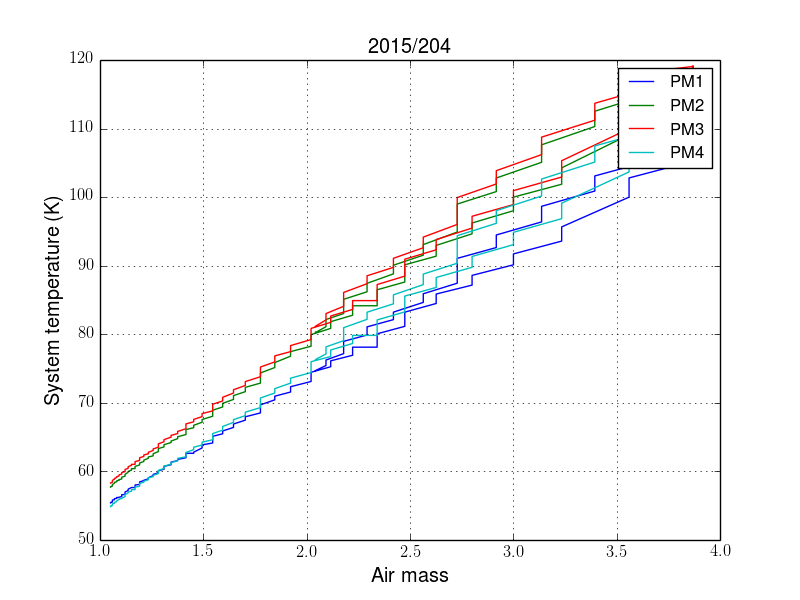
\includegraphics[width=5in]{tipping43-204-2.png}
\caption{\label{fig:tc-plot}Data from the first tipping curve on 2015/204.}
\end{center}
\end{figure}
The quality is good and so there is no need to extract a subset for fitting,
which is shown in Snippet~\ref{cod:tipfit}.
\begin{code}[h!tb]
\begin{center}
{\scriptsize \begin{verbatim}
In [8]: from DatesTimes import UnixTime_to_datetime
In [15]: UnixTime_to_datetime(sa.examiners[0].tctables[0].header['UNIXTIME']).strftime("%Y/%j %H:%M")
Out[15]: '2015/204 21:54
In [3]: sa.examiners[0].tctables[0].fit_data()
Out[3]: 
({0: 35.859516,   1: 35.363167,    2: 35.920727,    3: 33.488853},
 {0:  0.26522738, 1:  0.31136668,  2:  0.32382384,  3:  0.31152838},
 {0:  0.07538555, 1:  0.086743080, 2:  0.087312553, 3:  0.08278944},
 {0:  0.00048351, 1:  0.000567621, 2:  0.000590331, 3:  0.00056792},
 {}, {})\end{verbatim}
}\caption[Fit temperature {\itshape vs} airmass]{\label{cod:tipfit}Fitting 
TIPPING CURVE data to a straight line of system temperature {\itshape vs} 
airmass.}
\end{center}
\end{code}
The first row is the zero airmass system temperature and the second is its
standard deviation. The third row is the zenith optical depth and the fourth its
standard deviation. Two empty Python {\ttfamily dict}s are for the physical
temperature of the atmosphere along the line of sight if a quadratic fit is
done. (Usually not a good idea with 22~GHz data.)


\chapter{Plotting}\label{chap:plotting}

As explained in the previous chapter, initializing a {\ttfamily SessionAnalyzer}
class also creates a {\ttfamily DSNFITSplotter} object which adds plotting
capability.

\section{Class {\ttfamily DSNFITSplotter}}\label{sec:plotter}

{\ttfamily DSNFITSplotter} is actually a subclass of ({\itshape i.e.} is
derived from) {\ttfamily DSNFITSexaminer}, to which it adds plotting capability.
The real work of data reduction is done by {\ttfamily DSNFITSexaminer}.
{\ttfamily DSNFITSplotter} only creates a private class {\ttfamily Plotter}
object for each SINGLE DISH extension in the file.

 has one method:
\begin{description}\itemsep0pt \parskip0pt \parsep0pt
\item [plot\_average()] plots a DSN FITS spectrum averaged over the SINGLE DISH
tables in the file.  A DSN FITS spectrum is multi-dimensional with axes::
    [[beam,] [time,]], pol, [dec, RA], frequency-like
[] indicates the axes may not be present.  During data manipulations the
[ra, dec,] axes are the first to be eliminated.
    
Note that the frame of the provided spectrum is not changed.  Only the
X-axis is recomputed before plotting.
\end{description}


\subsection{Class {\ttfamily Plotter}}

The {\ttfamily Plotter} class has these methods:
\begin{description}\itemsep0pt \parskip0pt \parsep0pt
\item[figure\_rows\_and\_columns()] computes number of rows and columns for 
subplots.
\item[init\_multiplot()] creates a figure with multiple plots sharing common X 
and Y axis. The sublots have no space between them.
\item[init\_multiplots()] creates multiple figures with multiple plots.  The 
subplots have no space between the axes in a figure. Use
{\ttfamily figure\_rows\_and\_columns()} to compute number of figures, rows, 
columns and figure size.
\item[show\_passband()] creates dynamic spectra of the IFs. If there are multiple
beams, there will be a figure column for each beam and each pol.  Else, if there
is only one beam but multiple subchannels then there will be a figure column for
each subchannel and each pol. Otherwise there is just a column for each pol.
\item[show\_all\_spectra()] plots all the spectra in a table.  In each subplot are
all the spectra for each beam and polarization from one row in the SINGLE DISH
table. If there are multiple records in a row ({\itshape i.e.} a TIME dimension 
in DATA), all records are plotted (not the average over records).
\item[make\_legend\_labels()] is self-explanatory.
\item[plot\_BPSW\_spectra()] plots reduced beam and position switched spectra.
\item[plot\_PSSW\_spectra()] plots position switched spectra.
\item[plot\_line()] plots method reduced averaged spectral lines (from
{\ttfamily DSNFITSexaminer.Table} method {\ttfamily reduce\_line()}) for both 
pols.
\item[plot\_all\_Tsys()] displays all TSYS values so user can select row range.
(This works for WVSR data but needs work for SAO data.)
\item[plot\_Tsys()] plots average power versus time or airmass or list index.
\end{description}



\chapter{Programs}\label{chap:programs}

\section{Session Summaries}

describe

\section{Post-Processing}

Almost all observing sessions record data to intermediate data files.  These
files are converted to standard astronomical formats during or after the
observing session. The programs which perform these conversions are generally
run automatically.  Users can run them to regenerate the standard format files
as long as the original files are on-line.

\subsubsection{\ttfamily SAO2SDFITS}

describe

\section{Data Analysis}

\subsection{\ttfamily interactive.py}\label{sec:interact}

This program is a convenience for initializing the common data reduction classes
for analyzing the data from a session. Code Snippet~\ref{code:interactive} 
\begin{code}[h!tb]
\begin{center}
{\small \begin{verbatim}
kuiper@kuiper:...DSN-Sci-packages/Data_Reduction/FITS/apps/postproc$ ipython --pylab
...
In [2]: sa.examiners
Out[2]: {0: <Data_Reduction.FITS.SDFITSplotter.DSNFITSplotter at 0x7f3eb09ba0d0>}
In [3]: sa.examiners[0].tables
Out[3]: 
{0: <Data_Reduction.FITS.SDFITSexaminer.Table at 0x7f3eb091bad0>,
 1: <Data_Reduction.FITS.SDFITSexaminer.Table at 0x7f3eb08e1590>,
 2: <Data_Reduction.FITS.SDFITSexaminer.Table at 0x7f3eb08f7390>}
In [4]: sa.examiners[0].plotter
Out[4]: 
{0: <Data_Reduction.FITS.SDFITSplotter.Plotter at 0x7f3ea643ebd0>,
 1: <Data_Reduction.FITS.SDFITSplotter.Plotter at 0x7f3ea643eb90>,
 2: <Data_Reduction.FITS.SDFITSplotter.Plotter at 0x7f3ea643e410>}
In [5]: ex.tctables
Out[5]: 
{0: <Data_Reduction.FITS.SDFITSexaminer.TidTipAnalyzer instance at 0x7f3eb019bd40>,
 1: <Data_Reduction.FITS.SDFITSexaminer.TidTipAnalyzer instance at 0x7f3eb019bbd8>}
\end{verbatim}
}\caption[Program {\ttfamily interactive.py}]{\label{code:interactive}
Initiating a data reduction session with {\ttfamily interactive.py}.}
\end{center}
\end{code}
The {\ttfamily SDFITSexaminer.Table} and {\ttfamily SDFITSplotter} classes are 
decribed in section~\ref{sec:examiner} (page~\pageref{sec:examiner}).



\chapter{Monitor and Control System}\label{chap:MandC}

\section{Overview}

The DSN Radio Astronomy monitor and control system is designed for conducting
observations.  However, sometimes knowlege of the classes defined within the
M\&C system and their attributes ({\itshape i.e.} variables) and methods
({\itshape i.e. functions}) is helpful for analyzing data. This chapter touches
on the relevant features.

\appendix


\chapter{Workstation Configuration}\label{app:ws-configure}

To be done as {\ttfamily root}.  The secure way to do that is to be in the
{\ttfamily sudoers} file with ALL privilege. Then do
{\ttfamily sudo su -}.  The reason for doing this instead of prefixing all the
commands with {\ttfamily sudo} is that paths and permissions are different and
some commands may croak at installing files in some places.
\begin{verbatim}
apt-get install mlocate
apt-get install git
apt-get install apache2 php5 libapache2-mod-php5
apt-get install pyro
apt-get install python-setuptools
apt-get install python-pip
apt-get install python-epydoc
pip install dill
pip install pyephem
pip install openpyxl==1.5.8\end{verbatim}
The purposes of all these are:
\begin{description}\itemsep0pt \parskip0pt \parsep0pt
\item [mlocate] to build and maintain a searchable database of files.
\item [git] for software management.
\item [apache2] for web-based interfaces to the equipment servers.
\item [pyro] for inter-process communication in Python.
\item [setuptools] to facilitate packaging and installing Python projects.
\item [pip] to install and maintain packages in the Python Package Index.
\item [epydoc] for documenting Python source code.
\item [dill], a superior version of {\ttfamily pickle} with less restrictions.
\item [pyephem] to provide a superclass for {\ttfamily DSS} in
{\ttfamily Configurations}.
\item [openpyxl] to use Excel spreadsheets for configuration information and
data.
\end{description}

When these packages are installed one can bring in the Python monitor and
control software. All locally developed packages are in
{\ttfamily /usr/local/lib/python2.7/DSN-Sci-packages/}.  To put this directory
in the Python path the file {\ttfamily DSN-Sci-packages.pth} is put into\linebreak
{\ttfamily /usr/local/lib/python2.7/dist-packages}.  It contains one line:
\begin{verbatim}
kuiper@kuiper:/usr/local/lib/python2.7/dist-packages$ cat DSN-Sci-packages.pth
/usr/local/lib/python2.7/DSN-Sci-packages\end{verbatim}

The primary Git remote is at 
{\ttfamily https://ra.jpl.nasa.gov/}.  This is a password-protected remote
which can be used by our overseas partners who have access to the JPL domain
but not {\ttfamily github.jpl.nasa.gov} because they are not ``US persons''.

Because Gitlab does not support {\ttfamily gh-pages}, a method for publishing
web pages for a package, we also use, for now, {\ttfamily github.jpl.nasa.gov}
to provide these pages.

In the examples below, note the directories in which the repos are cloned.
This applies to all DSN Radio Astronomy hosts. The directory
{\ttfamily /usr/local} must be recursively writable by group {\ttfamily JPLusers}.
For setting up ssh tunnels and to provide a customized
version of {\ttfamily epidoc}.  
\begin{verbatim}
/usr/local/$ git clone https://ra.jpl.nasa.gov/RadioAstronomy/scripts.git\end{verbatim}
\noindent Package {\ttfamily support} provides a variety of general purpose modules.
\begin{verbatim}
/usr/local/lib/python2.7/DSN-Sci-packages$ git clone \
                           https://ra.jpl.nasa.gov/RadioAstronomy/support.git\end{verbatim}
\noindent For date and time conversions, probably needed for writing data files,
\begin{verbatim}
/usr/local/lib/python2.7/DSN-Sci-packages$ git clone \
                         https://ra.jpl.nasa.gov/RadioAstronomy/DatesTimes.git\end{verbatim}
\noindent The core of the monitor and control package is {\ttfamily MonitorControl}:
\begin{verbatim}
/usr/local/lib/python2.7/DSN-Sci-packages$ git clone \
                     https://ra.jpl.nasa.gov/RadioAstronomy/MonitorControl.git\end{verbatim}

Most servers manage some kind of equipment for which there are packages in
\begin{verbatim}
/usr/local/lib/python2.7/DSN-Sci-packages$ git clone \
                        https://ra.jpl.nasa.gov/RadioAstronomy/Electronics.git\end{verbatim}

As described in {\ttfamily https://github.jpl.nasa.gov/pages/RadioAstronomy/Overview/},
modules to support specific hardware are in sub-directories.  Only those modules
required for the hardware attached to the server need to be installed.  For
example, for Radipower power meters:
{\small \begin{verbatim}
/usr/local/lib/python2.7/DSN-Sci-packages/Electronics/Instruments$ git clone \
        https://ra.jpl.nasa.gov/kuiper/Electronics_Instruments_Radipower.git Radipower\end{verbatim}
}\noindent Note the difference with respect to the earlier clones:
\begin{itemize}\itemsep0pt \parskip0pt \parsep0pt
\item The {\ttfamily clone} is done in a sub-directory of the top-level repo
{\ttfamily Electronics}.
\item It is cloned into a sub-directory named for the last part of the repo name.
\end{itemize}
\noindent The repo names reflects the directory structure 
{\ttfamily Electronics/Instruments/Radipower} as well as the Python module 
import path {\ttfamily Electronics.Instruments.Radipower}

The configuration information for the DSN Complex where the server is
to be installed must also be cloned. For example
{\small \begin{verbatim}
/usr/local/lib/python2.7/DSN-Sci-packages/MonitorControl/Configurations$ git clone \
  https://ra.jpl.nasa.gov/RadioAstronomy/MonitorControl_Configurations_CDSCC.git CDSCC
\end{verbatim}
}\noindent


\chapter{Un Soup\c{c}on de Python}\label{Python}

The DSN Radio Astronomy Monitor and Control system uses the object-oriented
features of Python.  Arguably, object-oriented program can be said to be based
on Plato's theory of forms.  Python objects are analogous to real objects
while classes correspond to forms or ideals, which are abstractions based on
real objects.

\section{\ttfamily iPython}

One can simply type {\tt python} at a shell prompt to get the standard Python
command line interface.  However, {\tt ipython} is preferable because it has
powerful extra features.  One that is used most often is {\it tab completion}
illustrated in Snippet~\ref{code:tab}.
\begin{code}[h!tb]
\begin{center}
\begin{verbatim}
In [12]: sa.<Tab>
sa.DOY                    sa.get_good_weather_data  sa.project
sa.DSS                    sa.get_sources            sa.projectdatapath
sa.consolidate            sa.logger                 sa.projworkpath
sa.datapath               sa.open_datafiles         sa.sources
sa.examiner_keys          sa.plot_elev_and_Tsys     sa.year
sa.examiners              sa.plot_weather           
sa.get_average            sa.plot_wind\end{verbatim}
\caption[{\ttfamily ipython} tab completion]{\label{code:tab}Use of
{\ttfamily <Tab>} to see the names of an object's attributes and methods.}
\end{center}
\end{code}
This is very useful if you can't remember the name of an attribute or method.


\section{Classes}

A class is a natural way 
of describing a real-world object which has properties ({\it attributes}) and can
do things ({\it methods} or functions). 
The most basic class in the M\&C system is {\tt Device} which has the attributes 
{\tt name}, {\tt inputs} and {\tt outputs}, which are instance of {\tt Port}
classes, and {\tt data} about the device, such as the location of a telescope
or the bandwidth of a receiver.  Most classes discused here are sub-classes of 
{\tt Device}, which means that they ``inherit'' these attributes.

In the hope that it is more enlightening than confusing, 
Snippet~\ref{code:classTelescope} (page~\pageref{code:classTelescope}) gives an
example of a class definition.
\begin{code}[h!tb]
\begin{center}
\begin{verbatim}
  
class Telescope(Device):
  def __init__(self, obs, dss=0, LO=None, active=True):
    name = "DSS-"+str(dss)
    Device.__init__(self, name)
    self.inputs = {obs.name:obs}
    self['longitude'], self['latitude'], self['elevation'], tz, name, diam = \
            get_geodetic_coords(dss=int(dss))
    self['geo-x'],self['geo-y'],self['geo-z'] = \
            get_cartesian_coordinates('DSS '+str(dss))
    self.outputs[self.name] = Port(self, self.name, signal=Beam(str(dss)))
    self.outputs[self.name].signal['dss'] = dss\end{verbatim}
\caption{\label{code:classTelescope}Stripped-down definition of the 
{\tt Telescope} class.}
\end{center}
\end{code}
The {\tt \_\_init\_\_()} method creates an instance of this 
class\footnote{Creating an object from a class is called {\it instantiation},
making an {\tt instance} of a class.}, which 
inherits attributes from the class {\tt Device}. The second line creates the 
object and the rest of the code assigns values to its attributes.


\chapter{Polarization}\label{app:pol}

The DSN receivers are the older three-channel radio astronomy K-band receivers
have native circular polarization.  The default polarization of the new
four-channel K-band receiver is linear. In order to average gain variations in
the receiver channels over both measured polarizations, it is sometimes
desirable to convert from one polarization mode to the other. This appendix
gives the official definition of circular polarization and the technique for
changing polarization mode.

\section{IAU Definition of Circular Polarization}

As reported in the Proceedings of the Fifteenth General Assembly \cite{IAU1974},
the following resolution was adopted by IAU Commissions 25 (Stellar Photometry
and Polarimetry) and 40 (Radio Astronomy):

{\itshape RESOLVED, that the frame of reference for the Stokes parameters is
that of Right Ascension and Declination with the position angle of the
electric-vector maximum, $\theta$, starting from North and increasing through
East. Elliptical polarization is defined in conformity with the definitions of
the Institute of Electrical and Electronics Engineers
(IEEE Standard 211)}\cite{IEEE1969}.

{\bfseries Left-Handed (Counterclockwise) Polarized Wave} (LCP):
An elliptically polarized electromagnetic wave in which the
rotation of the electric field vector with time is
counterclockwise for a stationary observer looking in the
direction of the wave normal.

{\bfseries Right-Handed (Clockwise) Polarized Wave} (RCP): 
An elliptically polarized electromagnetic wave in which the
rotation of the electric field vector with time is clockwise
for a stationary observer looking in the direction of the wave
normal.

This means that the polarization of incoming radiation for which the position
angle of the electric vector measured at a fixed point in space
increases with time is described as right-handed and positive.
\begin{figure}[h!tb]
\begin{center}
\includegraphics[width=4in]{circular.png}
\caption[Circular Polarization]
{\label{fig:circ_pol} A right circularly polarized wave (LCP - green) and left
circularly polarized wave (RCP - red)
as defined by the IAU are shown decomposed into two
orthogonal linearly polarized waves (X - magenta, Y - blue). The thick arrows
show the direction of propagation.}
\end{center}
\end{figure}
This can be seen in the lower panel of Figure~\ref{fig:circ_pol}\footnote{To 
view these images relax the eye muscles as if
looking at a distant object. A person not experienced in this
type of viewing might first look at a distant object and then
slide the gaze down to the figure without refocusing. Another
method is to place a sheet of cardboard with one edge down the
middle of the figure and the other edge between the eyes. It is
probably easier to focus first on a label above or below
the spiral, and then slide the gaze downwards.}

\section{Changing Between Linear and Circular
Polarization}\label{sec:lin-circ}

Figure~\ref{fig:circ_pol} shows that linear polarization can be converted to 
circular polarization.  If the vertical (H-plane or Y-axis) wave lags
behind the horizontal (E-plane or X-axis) wave by $90^{\circ}$ of
phase delay the resulting polarization will be RCP.
If the vertical (H-plane or Y-axis) wave leads
the horizontal (E-plane or X-axis) wave by $90^{\circ}$ of
phase delay the resulting polarization will be LCP.

Optically, this can be accomplished
by passing the beam through a particular thickness of material which
has different indices of refraction for two orthogonally polarized
components. Similarly, a waveguide section can be produced to perform the
same function.

\begin{figure}[h!tb]
\begin{center}
\includegraphics[width=3.5in]{quad_hybrid.png}
\caption[Quadrature hybrid]{\label{fig:quad-hybrid}A quadrature hybrid
combines two input signals so that one is delayed $90^{\circ}$
with respect to the other. There are two outputs which are
symmetrically delayed.  The figure on the left shows a
conventional schematic.  The one on the right is a more
illustrative schematic.}
\end{center}
\end{figure}
In the cm, mm, and submm wave domains, there exist devices which can
separate a radio wave into two orthogonally polarized components.
A quadrature hybrid can convert between the two modes, as shown in
Figure \ref{fig:quad-hybrid}. If port A were receiving
vertical polarization (H-plane or Y-axis) and B horizontal polarization 
(E-plane or X-axis) then at the port labelled A+$\angle 90^{\circ}$B, the
vertical polarization lags behind the horizontal and it would put out RCP.
The port labelled B+$\angle 90^{\circ}$A would put out LCP.

From this one can see that, if there is an option to bypass the hybrid, it 
depends which way the hybrid is put in the 
circuit which determines whether the output ports are E/L and H/R or are
E/R and H/L.

\chapter{Sideband Separation}\label{app:complex}


If the LO is in the middle of the RF band, then the mixing products will have
both positive frequencies from the upper sideband and negative frequencies from
the lower sideband. Both are present in the IF.  A complex mixer puts out
two IFs which are separated 90$^{\circ}$ in phase.  These two IFs can be
considered the real and imaginary parts of a complex signal. The upper and
lower sidebands can be recovered from a complex signal.

The outputs from a complex mixer can be phased together to separate
the upper and lower sidebands.  This is done with a $90^{\circ}$ hybrid,
shown in Figure~\ref{fig:quad-hybrid},
which re-combines the two quadrature phase mixing products.
To see this, consider the outputs of the two mixers to be the sum of
the USB and the LSB part of the down-converted spectrum with the
frequencies explicitly positive and negative,
{\itshape i.e.},
\begin{eqnarray}
V_R &=&   \frac{V_{U}}{\sqrt{2}} \cos( \omega_{U} t + \Delta \phi_{U})
        + \frac{V_{L}}{\sqrt{2}} \cos(-\omega_{L} t + \Delta \phi_{L}),
          \label{eq:V_real-1} \\
    &=&   \frac{V_{U}}{\sqrt{2}} \cos(\omega_{U} t + \Delta \phi_{U})
        + \frac{V_{L}}{\sqrt{2}} \cos(\omega_{L} t - \Delta \phi_{L}),
          \label{eq:V_real-2} \\
V_I &=&   \frac{V_{U}}{\sqrt{2}} \sin( \omega_{U} t + \Delta \phi_{U})
        + \frac{V_{L}}{\sqrt{2}} \sin(-\omega_{L} t + \Delta \phi_{L}),
          \label{eq:V_imag-1} \\
    &=&   \frac{V_{U}}{\sqrt{2}} \sin(\omega_{U} t + \Delta \phi_{U})
        - \frac{V_{L}}{\sqrt{2}} \sin(\omega_{L} t - \Delta \phi_{L})
      \label{eq:V_imag-2}
\end{eqnarray}
where $U$ refers to the upper sideband and $L$ the lower sideband.
Then if these signals are combined in a quadrature hybrid, the effect
along the paths with the $\pi/2$ delay is that the delayed signal at
the summation point is that which entered the delay section $t - \pi/2\omega$
earlier.  This means that we subtract $\pi/2$ from the angular terms in 
Equations~\ref{eq:V_real-1} and~\ref{eq:V_imag-1} as illustrated
in Figure~\ref{fig:phase-delay}.
\begin{figure}[h!tb]
\begin{center}
\includegraphics[width=5in]{hybrid-delay.png}
\caption[Phase delay]{\label{fig:phase-delay}The angular term for the green line
in the lower panel is $\pi/2$ smaller than in the upper panel, showing that the
effect is to delay the signal. (The dotted
lines show a slighly earlier time for a positive frequency signal; so
the signal moves left with time.)}
\end{center}
\end{figure}

Subtracting $\pi/2$ from the angular terms is equivalent to 
subtracting $\pi/2$ from the phases associated with the positive 
frequency terms and adding $\pi/2$ to the phases associated with the 
negative frequency terms in Equations~\ref{eq:V_real-2} and~\ref{eq:V_imag-2}.
The outputs from the hybrid will then be
\begin{eqnarray}
\frac{V_R}{\sqrt{2}} + \frac{V_I \angle 90^{\circ}}{\sqrt{2}} \label{eq:sum_usb}
&=&
   \frac{V_{U}}{\sqrt{2}} \cos(\omega_{U} t + \phi_{U})
 + \frac{V_{L}}{\sqrt{2}} \cos(\omega_{L} t - \phi_{L}) \nonumber \\
& &
  + \frac{V_{U}}{\sqrt{2}} \sin(\omega_{U} t + \phi_{U} - \frac{\pi}{2})
  - \frac{V_{L}}{\sqrt{2}} \sin(\omega_{L} t - \phi_{L} - \frac{\pi}{2})
     \nonumber \\
&=&
\;\;  \frac{V_{U}}{\sqrt{2}} \cos(\omega_{U} t + \phi_{U})
    + \frac{V_{L}}{\sqrt{2}} \cos(\omega_{L} t - \phi_{L})
\nonumber \\
& & - \frac{V_{U}}{\sqrt{2}} \cos(\omega_{U} t + \phi_{U})
    + \frac{V_{L}}{\sqrt{2}} \cos(\omega_{L} t - \phi_{L})
\nonumber \\
&=& \;\;   \sqrt{2}V_{L} \cos(\omega_{L} t + \phi_{L}) \label{eq:nu_usb}\\
\frac{V_R \angle 90^{\circ}}{\sqrt{2}} + \frac{V_I}{\sqrt{2}} \label{eq:sum_lsb}
&=&
   \frac{V_{U}}{\sqrt{2}} \cos(\omega_{U} t + \phi_{U} - \frac{\pi}{2})
 + \frac{V_{L}}{\sqrt{2}} \cos(\omega_{L} t - \phi_{L} - \frac{\pi}{2}) \nonumber \\
& &
 + \frac{V_{U}}{\sqrt{2}} \sin(\omega_{U} t + \phi_{U})
 - \frac{V_{L}}{\sqrt{2}} \sin(\omega_{L} t - \phi_{L})
     \nonumber \\
&=&
  \frac{V_{U}}{\sqrt{2}} \sin(\omega_{U} t + \phi_{U})
 + \frac{V_{L}}{\sqrt{2}} \sin(\omega_{U} t - \phi_{L})
\nonumber \\
& &    + \frac{V_{U}}{\sqrt{2}} \sin(\omega_{U} t + \phi_{U})
       - \frac{V_{L}}{\sqrt{2}} \sin(\omega_{U} t - \phi_{L})
\nonumber \\
&=& \!    \sqrt{2}V_{U} \sin(\omega_{U} t + \phi_{U})
\end{eqnarray}
Note that adding $\pi/2$ to the image band terms in
Equations~\ref{eq:V_real-1} and~\ref{eq:V_imag-1} is like subtracting
$\pi/2$ from the image band terms in
Equations~\ref{eq:V_real-2} and~\ref{eq:V_imag-2},
{\itshape i.e.} the sign of the $\pi/2$ added is the same as the sign
of the frequency.

The time-averaged power in each band is
\begin{eqnarray}
P_{USB} &=& V^2_{USB} \nonumber \\
        &=& 2 V^2_{U}
\left \langle\cos^2(\omega_{IF} t + \phi_{U}) \right \rangle
\nonumber \\
        &=& V^2_{U} \label{eq:usb_power}\\
P_{LSB} &=& V^2_{L} \label{eq:lsb_power}
\end{eqnarray}
Equations \ref{eq:usb_power} and \ref{eq:lsb_power},
when added together, give the power in both sidebands.


\bibliographystyle{apj}
\bibliography{Astronomy}
\clearpage

\printindex

\end{document}
